% version 1.00, date 12/05/16, auteur(s) Pierre Porche, Sergi Colomies
\documentclass[compress,xcolor=dvipsnames]{beamer}

%Pour les schémas d'architecture
\usepackage{etex}
\usepackage{tikz}
\usetikzlibrary{shapes,arrows,chains,backgrounds,fit}
%FIN Pour les shémas d'architecture

\usepackage[french]{babel}
\selectlanguage{french}
\usepackage[utf8]{inputenc}
\usepackage[T1]{fontenc}
\usepackage{tikz}
\usepackage{wrapfig}
\usepackage{multirow}
%\usepackage{pgf-pie}
\usepackage{pgfplots}
\usepackage{pdfpages}
\usepackage{vocabulaireUnipikPresentation}
\usepackage{commun/vocabulaireCommun}
\usepackage{hyperref}
\usepackage{movie15}
\usepackage{xcolor}
\usepackage{lscape}
\usepackage{booktabs}
\usepackage{multirow}
\usepackage{colortbl}

\newcommand{\tabincell}[2]{\begin{tabular}{@{}#1@{}}#2\end{tabular}}

\usetheme{eastpic}%{Berlin}%{Madrid}

 
 
%Information to be included in the title page:
\title{Revue de PIC}
\date{\today}
\author{Unipik}
\institute{\insa}

\setbeameroption{show notes}

 
\begin{document}

\speaker{\Sergi} 

\begin{frame}[plain]
	\titlepage
\end{frame}

\begin{frame}{Sommaire}
	\tableofcontents[hideallsubsections]
\end{frame}
 

\speaker{\Sergi}
\section[Présentation]{Présentation}
\subsection{} % PAs besoin de titre

\begin{frame}
\frametitle{Présentation de l'équipe}
	\begin{figure}
		\includegraphics[scale=0.25]{images/organigrammeFonctionnel.png}
		\caption{Organigramme fonctionnel}
		\label{OF}
	\end{figure}
\end{frame}

\speaker{Mélissa Bignoux}
\begin{frame}
\frametitle{Présentation du client}
	\begin{center}
		UNICEF
	\end{center}
	\begin{itemize}
		\item Un des principaux organismes d’aide humanitaire et de développement
		\item Acteur partout dans le monde en faveur des droits de chaque enfant
	\end{itemize}
	
	\begin{center}
		UNICEF Seine-Maritime
	\end{center}
	Ses actions principales sont : 
	\begin{itemize}
		\item La sensibilisation aux droits de l'enfant
		\item Les événements 
		\item Les ventes sur stands
	\end{itemize}
	
\end{frame}
\speaker{Mélissa Bignoux}
\begin{frame}
\frametitle{Présentation du sujet}
Outil de gestion informatique des interventions externes suivantes :

	\begin{itemize}
		\item Les plaidoyers dans les \'ecoles
		\item Les actions frimousses
		\item Les projets de lycéens et d'étudiants
		\item Les actions ponctuelles
	\end{itemize}
	
\end{frame}


\section[Avancement]{Avancement du Projet}
% version 1.00, date 07/03/16, auteur Matthieu Martins-Baltar
%\subsection{} % Pas besoin de titre


\subsection{Introduction}
%version 1.00,	date 19/10/2016	auteur(s) François Decq
\speaker{\Francois}

\begin{frame}
\frametitle{Rappels}
\begin{block}{Technologies}
	\begin{itemize}
		\item Symfony3 : framework PHP
		\item Base de données : PostgreSql
		\item ORM : Doctrine
		\item Moteur de templates : TWIG
	\end{itemize}
\end{block}
\end{frame}

\begin{frame}
\frametitle{Rappels}
\begin{block}{Fin du semestre dernier : lot 1}
	\begin{itemize}
		\item L'architecture du projet est finalisée
		\begin{figure}[!h]
			\begin{center}
				\includegraphics[scale=0.25]{images/mvcGeneral.pdf}
				\caption{Patron de conception MVC}
			\end{center}
		\end{figure}
		\item L'architecture de la base de données est stable
	\end{itemize}
\end{block}
\end{frame}

\subsection{Conception BD}
\speaker{\Michel}

\begin{frame}
\frametitle{\underline{M}VC : Le modèle}
\begin{figure}[!h]
	\begin{center}
	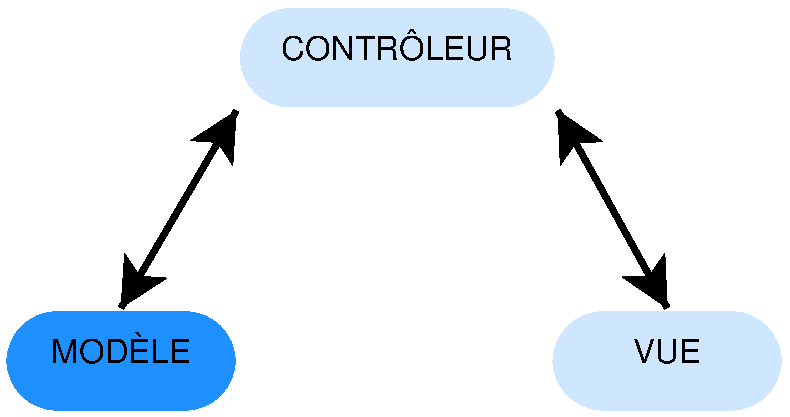
\includegraphics[scale=0.5]{images/mvcModele}
	\caption{Architecture \underline{M}VC}
	\end{center}
\end{figure}
\end{frame}

%%%%%%%%%%%%%%%%%%%%%%%%%%%%%%%%%%%%%%%%%%%%%%%%%%%

\begin{frame}
	\frametitle{\underline{M}VC : Le modèle}
	\begin{block}{Modélisation de la Base de Données}	
		\begin{itemize}
			\item Réalisation du diagramme de classes
			\item Création de la Base de Données et mapping avec les entités du projet grâce à notre ORM Doctrine
		\end{itemize}
	\end{block}
\end{frame}

%%%%%%%%%%%%%%%%%%%%%%%%%%%%%%%%%%%%%%%%%%%%%%%%%%%

\begin{frame}
	\frametitle{\underline{M}VC : Le modèle}
	\begin{block}{Mapping entre les classes PHP et la Base de Données}	
		\begin{columns}
			\begin{column}{0.9cm}
			\end{column}
			\begin{column}{6cm}
				\begin{Large} Top Down\end{Large}
				\begin{itemize}
					\item Approche descendante
					\item Système d'annotation dans les classes PHP
					\item Génération des tables de la Base de Données
				\end{itemize}
		\end{column}
		
		\begin{column}{4cm}
			\begin{figure}[!h]
				\begin{center}
					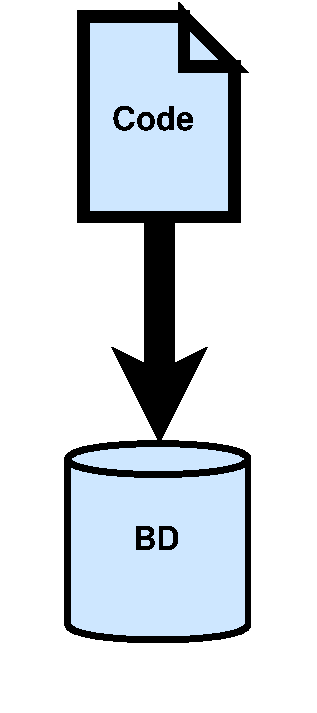
\includegraphics[scale=0.275]{images/topDown}
					\caption{Top Down}
				\end{center}
			\end{figure}
		\end{column}
	
	\end{columns}
	\end{block} 
\end{frame}

\begin{frame}
	\frametitle{\underline{M}VC : Le modèle}
	\begin{block}{Mapping entre les classes PHP et la Base de Données}	
		\begin{columns}
			\begin{column}{0.9cm}
			\end{column}
			\begin{column}{6cm}
				\begin{Large}Bottom Up\end{Large}
				\begin{itemize}
					\item Approche ascendante
					\item Création de la Base de Données
					\item Génération des fichiers de mapping et classes PHP
				\end{itemize}
			\end{column}
			
			\begin{column}{4cm}
			\begin{figure}[!h]
				\begin{center}
					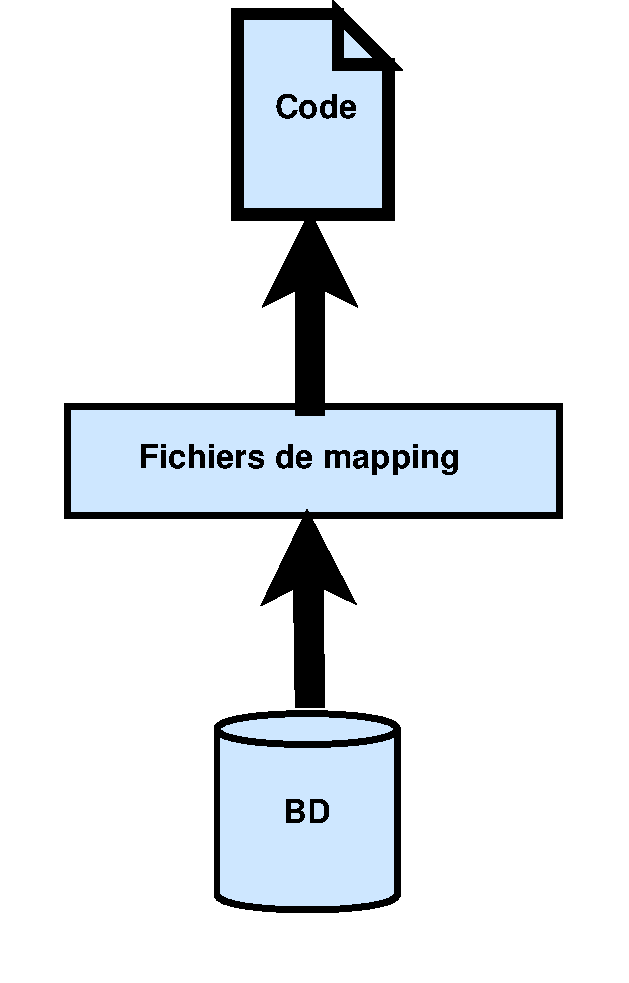
\includegraphics[scale=0.225]{images/bottomUp}
					\caption{Bottom Up}
				\end{center}
			\end{figure}
		\end{column}
	
	\end{columns}
	\end{block} 
\end{frame}



%%%%%%%%%%%%%%%%%%%%%%%%%%%%%%%%%%%%%%%%%%%%%%%%%%%

\speaker{\Julie}
\begin{frame}
	\frametitle{\underline{M}VC : Le modèle}
	\begin{block}{Top Down}
		Avantages :
		\begin{itemize}
			\item Approche objet
			\item Doctrine initialement prévu pour une approche Top Down
		\end{itemize}
 
		Inconvénients :
		\begin{itemize}
			\item Non visibilité du cycle de vie
			\item Création d'une table intermédiaire pour les attributs multivalués
			\item Mauvaise gestion de l'héritage
			\item Mauvaise gestion des attributs d'association
			
		\end{itemize}
	\end{block}
\end{frame}


%%%%%%%%%%%%%%%%%%%%%%%%%%%%%%%%%%%%%%%%%%%%%%%%%%%

\begin{frame}
	\frametitle{\underline{M}VC : Le modèle}
		\begin{figure}[!h]
			\begin{center}
				\includegraphics[scale=0.225]{images/explicationProblemeBD}
				\caption{Mauvaise gestion des attributs d'association}
			\end{center}
		\end{figure}
\end{frame}


%%%%%%%%%%%%%%%%%%%%%%%%%%%%%%%%%%%%%%%%%%%%%%%%%%%

\begin{frame}
	\frametitle{\underline{M}VC : Le modèle}
	\begin{block}{Bottom Up}
	Avantages :
		\begin{itemize}
			\item Propreté de la Base de Données
			\item Amélioration des performances
			\item Vérification des contraintes dans la Base de Données
		\end{itemize} 
	Inconvénients :
		\begin{itemize}
			\item ORM non adapté
			\item Vérification et modification d'une partie des fichiers générés
		\end{itemize}
	\end{block}
  
\end{frame}

%%%%%%%%%%%%%%%%%%%%%%%%%%%%%%%%%%%%%%%%%%%%%%%%%%%

\begin{frame}
	\frametitle{\underline{M}VC : Le modèle}
	\begin{block}{Décision : Bottom Up}
		\begin{itemize}
		\item Une bonne structure de base représente une anticipation des problèmes par la suite 
		\item Mieux adapté pour une possible utilisation au niveau Unicef France
		\end{itemize}
		
		
	\end{block}
\end{frame}





\subsection{Réalisation de vues}
\speaker{\Mathieu}

\begin{frame}
\frametitle{M\underline{V}C : Les vues}
\begin{figure}[!h]
	\begin{center}
	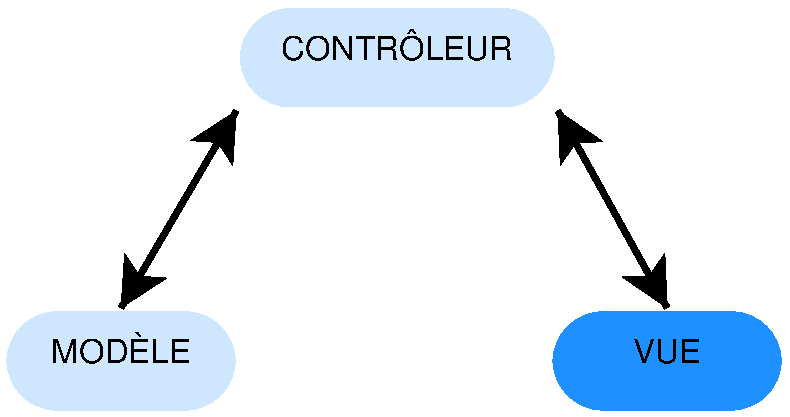
\includegraphics[scale=0.5]{images/mvcVue}
	\caption{Architecture M\underline{V}C}
	\end{center}
\end{figure}
Vue : partie visible, IHM(Interface Homme Machine)
\end{frame}

\begin{frame}
\frametitle{M\underline{V}C : Les vues}
\begin{block}{Vocabulaire}
\textbf{Template} : définit l'habillage d'une page, la position de ses éléments
\end{block}
\begin{figure}[!h]
	\begin{center}
	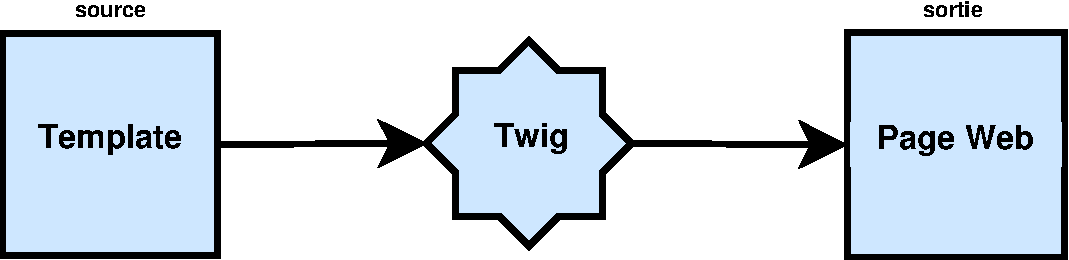
\includegraphics[scale=0.5]{images/twig}
	\caption{Fonctionnement du moteur de template Twig}
	\end{center}
\end{figure}
\end{frame}

\begin{frame}
\frametitle{M\underline{V}C : Les vues}
Architecture des templates :
\begin{itemize}
\item Niveau 1 : Architecture générale pour l'ensemble des pages
\item Niveau 2 : Architecture spécifique pour chaque groupe de pages similaires
\item Niveau 3 : Templates finaux pour chaque page Web de l'application
\end{itemize}
\begin{figure}[!h]
	\begin{center}
	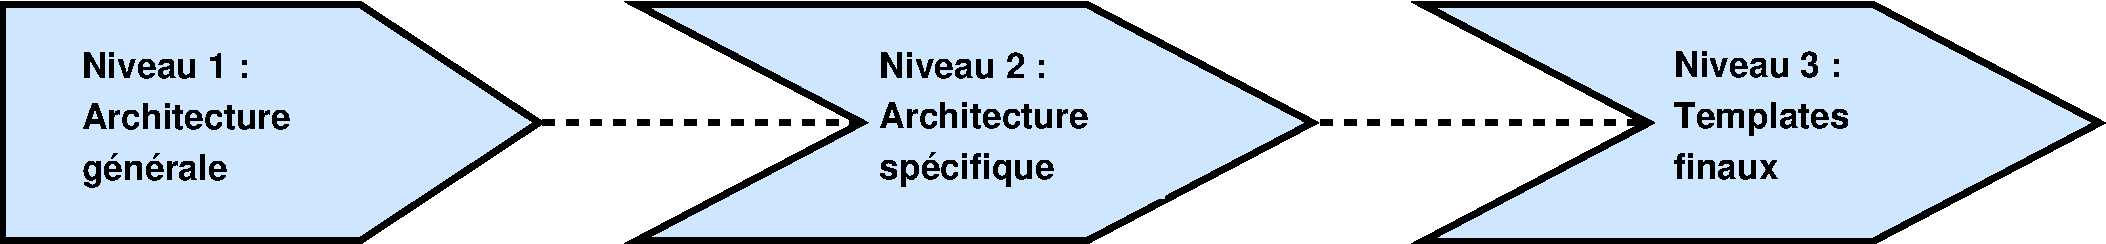
\includegraphics[scale=0.3]{images/archiTemplates}
	\caption{Imbrication des templates}
	\end{center}
\end{figure}
\end{frame}

\begin{frame}
\frametitle{M\underline{V}C : Les vues}
Utilisation d'une collection d'outils CSS : Bootstrap
\begin{itemize}
\item Gain de temps
\item Pris nativement en charge par Symfony
\item Permet d'avoir une application accessible depuis tout type d'appareil (ordinateur, tablette, smartphone)
\end{itemize}
\end{frame}

\begin{frame}
Affichage d'une vue
\end{frame}

\begin{frame}
Affichage d'une autre vue
\end{frame}


\subsection{Développement Contrôleur}
\speaker{\Florian}

%%%%%%%% Slide Bundle %%%%%%%%
\begin{frame}
  \frametitle{\underline{M}V\underline{C} : Les Bundles}   
\begin{figure}[!h]
	\begin{center}
	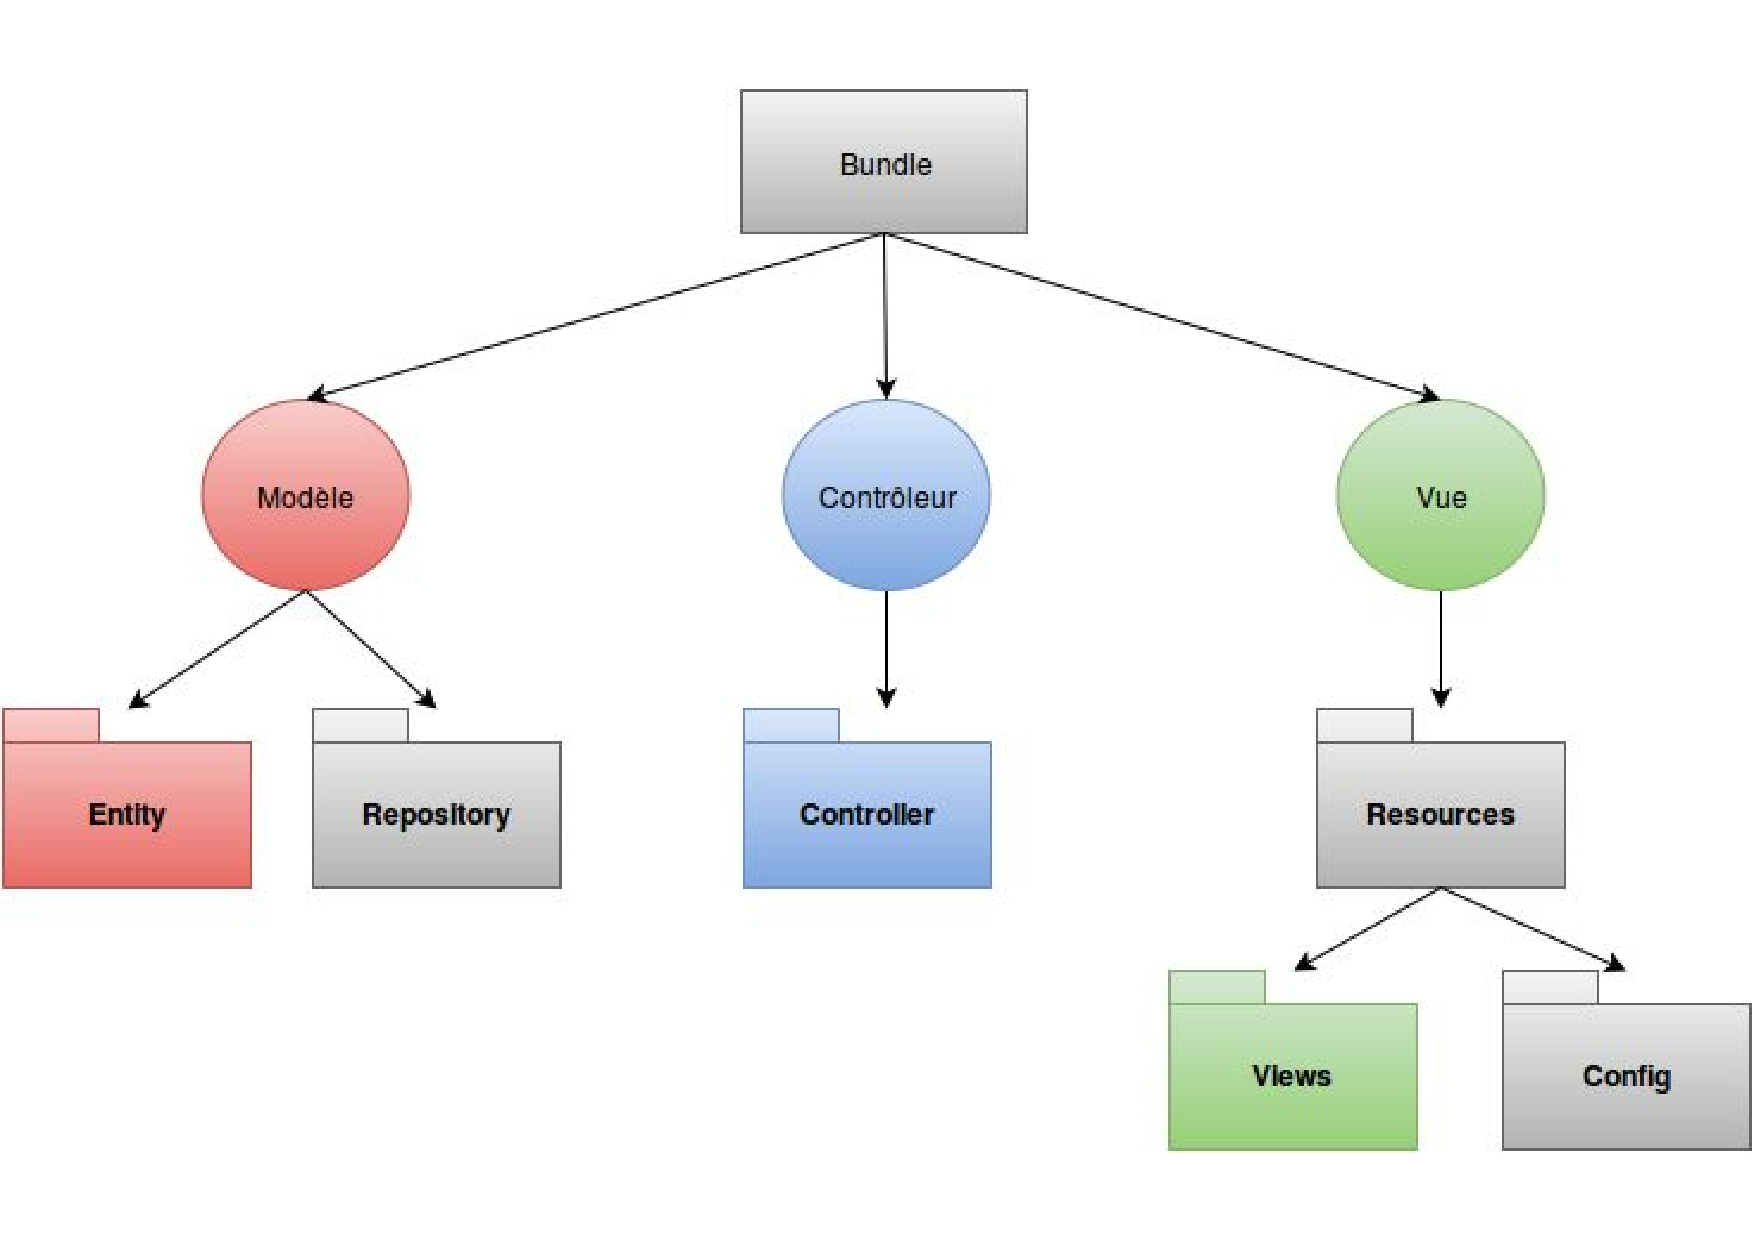
\includegraphics[scale=0.3]{images/bundles}
	\caption{Architecture \underline{M}V\underline{C}}
	\end{center}
\end{figure}
\end{frame}

%%%%%%%%%%% Slide fonctionnement %%%%%%%%

\begin{frame}
  \frametitle{\underline{M}V\underline{C} : Fonctionnement de l'application}
        \begin{figure}[!h]
	\begin{center}
	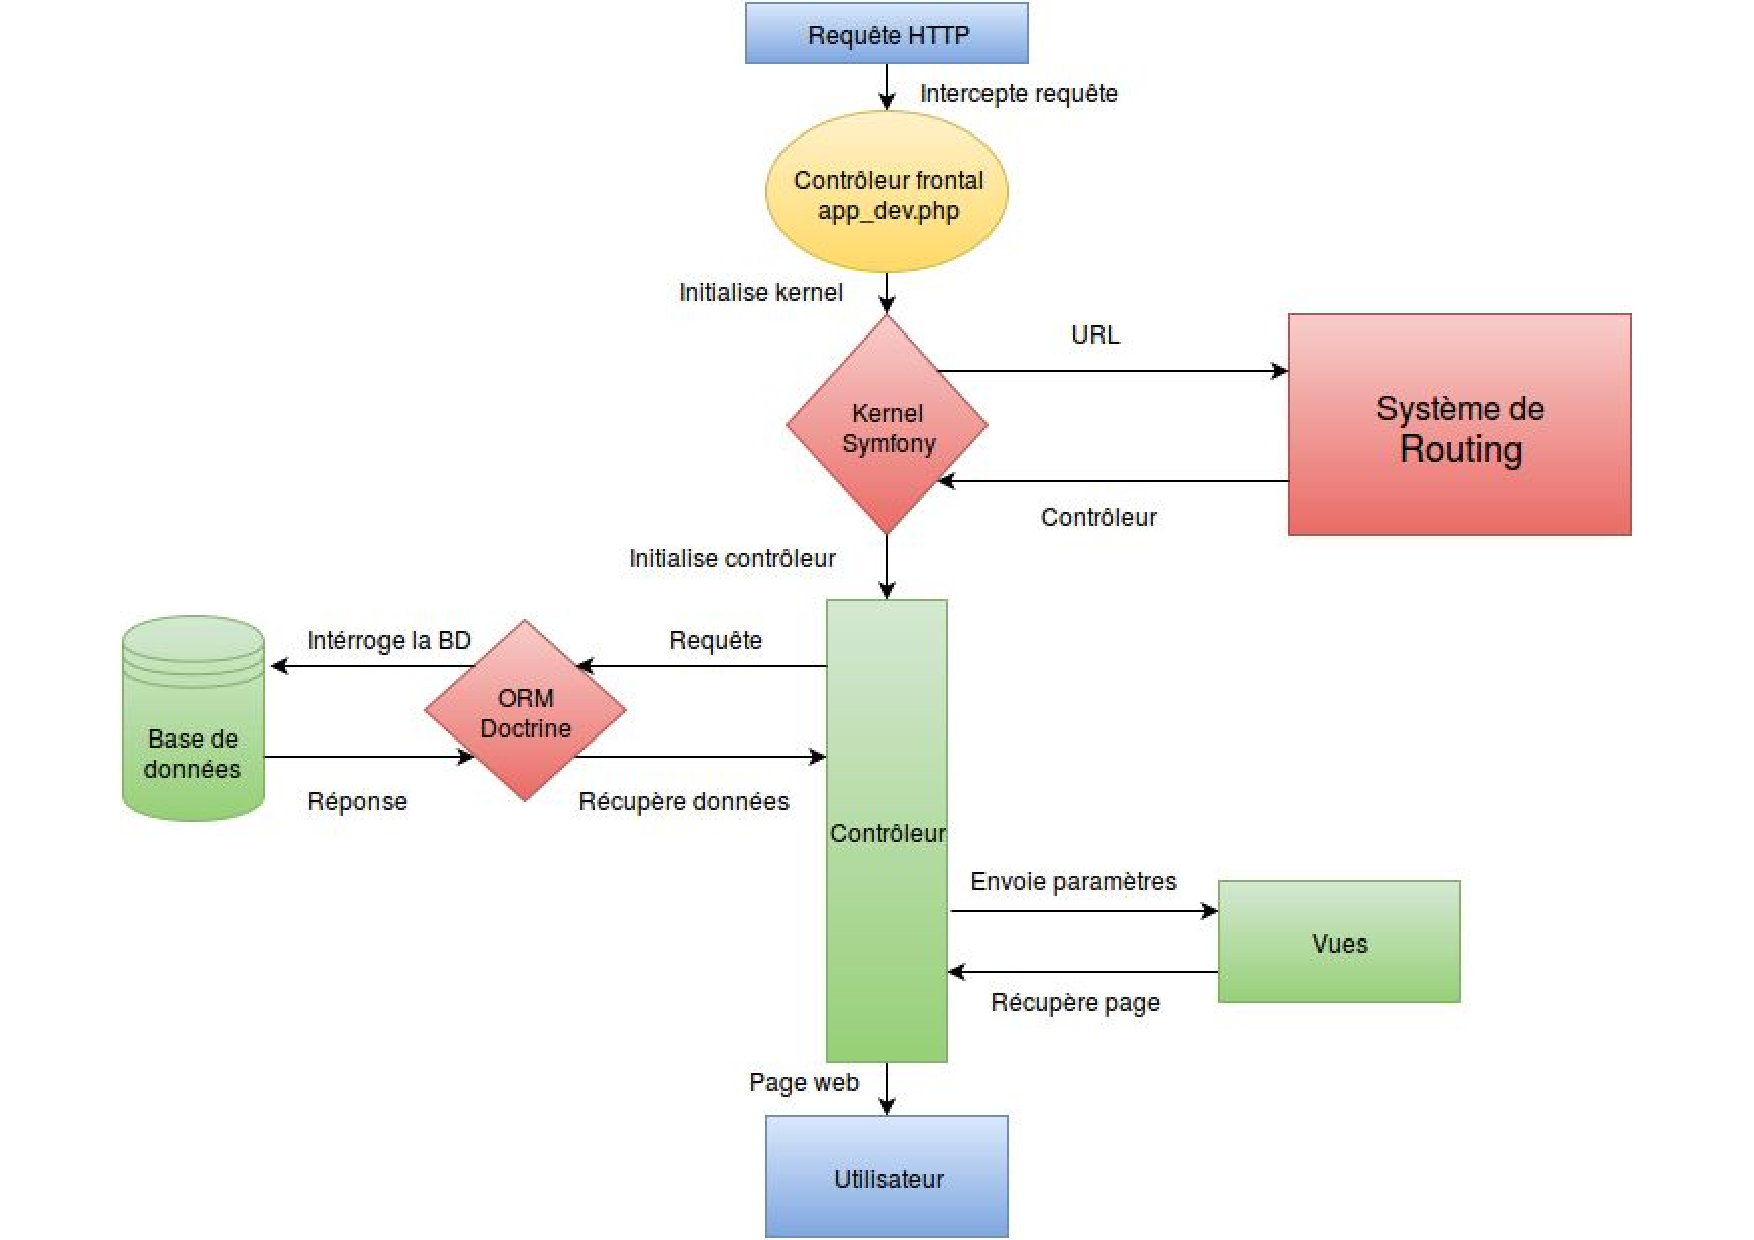
\includegraphics[scale=0.3]{images/symfony}
	\caption{Architecture \underline{M}V\underline{C}}
	\end{center}
\end{figure}
\end{frame}

%%%%%%%% Slide Nos Bundles %%%%%%%%%%

\begin{frame}
  \frametitle{\underline{M}V\underline{C} : Notre Architecture}
  \begin{block}{Nos Bundles}
  \begin{itemize}
  \item Bundle Utilisateur : gestion des comptes utilisateur
  \item Bundle Intervention : gestion des interventions menées par les bénévoles
  \item Bundle Mail : gestion de l'envoi des mails
  \item Bundle Architecture : gestion de la structure de l'application
  \end{itemize}
  \end{block}   
  \end{frame}

%%%%%%%% Slide User Bundle %%%%%%

\begin{frame}
\begin{block}{Bundle Utilisateur}
\frametitle{\underline{M}V\underline{C} : Le bundle utilisateur}
\begin{itemize}
\item Gestion des comptes utilisateurs
\item Création de compte
\item Envoi de mail contenant un lien d'activation
\item Mots de passe hashés et salés
\item Système d'authentification
\item Page de profil 
\end{itemize}
\end{block}
\end{frame}



\subsection{Avancement Serveur}
% version 1.00, date 10/05/16, auteur Matthieu Martins-Baltar


\speaker{\Matthieu}

\begin{frame}
	\frametitle{Serveur}
    Problématique du serveur :
      \begin{itemize}
        \item Projet nécessitant un serveur
        \item Client avec des ressources limitées
        \item Client non technique
      \end{itemize}
\end{frame}

\begin{frame}
	\frametitle{Serveur}
	Solution explorée jusque là :
	\begin{itemize}	
    \item Hébergement par l'INSA
    \end{itemize}
    
	Accord proposé :
	\begin{itemize}
		\item Mise en place d'un programme UNICEF Campus
		\item Création de Projets d’Ouverture et d’Approfondissement %nouvelles fonctionnalité et/ou admin sys
	\end{itemize}
\end{frame}

\begin{frame}
	 Rencontre avec de nombreux interlocuteurs :
	\begin{itemize}
    	\item Présentation de la problématique pour obtenir leur soutien:
		\begin{itemize}
			\item Anne Caldin (service culturel)
			\item Maxime Reynet (service com)
			\item Direction Générale (via Gilles Gasso)
		\end{itemize}
		\item Présentation du dossier avec les demandes techniques précises:
		\begin{itemize}
			\item Baptiste Blondel-Angot (service juridique)
			\item Laurent Vasseur et Sébastien Bonnegent (DSI)
		\end{itemize}    
	\end{itemize}    
\end{frame}

\begin{frame}
	Demandes techniques :
	\begin{itemize}
		\item serveur web Apache
		\item PHP 5.5.9 avec options (PHP-XML, PDO, etc.) 
		\item PostgreSQL + PostGIS (faible volumétrie)
		\item Paramètres divers (JSON, ctype, libxml, etc.)
	\end{itemize}

    Autres solutions possibles :
      \begin{itemize}
        \item Faire une demande de mécénat auprès d'un hébergeur privé
        \item Faire une demande auprès d'UNICEF France
        \item Envisager une solution payante, la moins chère possible
      \end{itemize}
\end{frame}





\section[Qualité]{Démarche Qualité}
%version 1.00,	date 12/05/2016	auteur(s) Pierre Porche

\speaker{\Pierre}

\subsection{} % PAs besoin de titre


\begin{frame}
\frametitle{Continuité dans la démarche Qualité}
Principe de l'amélioration continue :
\begin{itemize}
\item Suivi de la satisfaction client
\item Suivi de l'évolution des risques et opportunités
\item Mise à jour des documents de Qualité
\item Suivi de la traçabilité et sensibilisation de l'équipe
\end{itemize}
\end{frame}


\begin{frame}
\frametitle{Formation de l'équipe}
Montée en puissance avant atteinte des limites :
\begin{itemize}
\item Identification des compétences à développer
\item Planification des formations
\item Répartition des tâches de formation
\item Rédaction des documents de formation
\end{itemize}
\end{frame}


\begin{frame}
\frametitle{Audit interne de Qualité}
Le 15/03/2016 par \nomApprobateur{} et \nomTuteurQualite{} :
\begin{itemize}
\item Vérification du suivi de la norme ISO 9001 : 2015
\item Zéro non-conformité
\item Cinq remarques
\item Identification et correction de chaque \FT{} levé
\end{itemize}
\end{frame}







\section[Conduite du projet]{Conduite du Projet}
\subsection{} % PAs besoin de titre

\begin{frame}
\frametitle{UNICEF 76}
\framesubtitle{Les actions}
	\begin{itemize}
		\item Plaidoyers dans les \'ecoles
		\item Actions frimousses
		\item Villes Amies des Enfants
		\item Ventes ponctuelles
	\end{itemize}
\end{frame}


\section[Conclusion]{Conclusion}
%version 1.00,	date 12/05/2016	auteur(s) Pierre Porche



\subsection{} % PAs besoin de titre

\speaker{\Pierre}
\begin{frame}
\frametitle{Conclusion}
	Nos réussites :
	\begin{itemize}
		\item Etre Beaux
		\item Réussir le swag
	\end{itemize}
	
	Ce que le projet nous a apporté : 
	\begin{itemize}
		\item DU PAPIÉ GRATUI
		\item DES ANSSEINTTE KI METT DU SON 2 BANLIEU
	\end{itemize}
\end{frame}


\end{document}

